% !TEX TS-program = pdflatex
% !TEX encoding = UTF-8 Unicode

%\documentclass[ing,male,java,dept460,oneside]{diploma}
\documentclass{article}

\usepackage[czech]{babel}
\usepackage[T1]{fontenc}
\usepackage[utf8]{inputenc}
\usepackage{color}
\usepackage{geometry}
\usepackage{float}
\usepackage{graphicx}
\usepackage[stable]{footmisc}
\usepackage{hyperref}
\usepackage{amsfonts}
 \usepackage{bbm}
 \usepackage{booktabs}
 \usepackage{url}
 \usepackage{nameref}



% \ThesisAuthor{Josef Raška}

% U bakalarske praxe neni nutne nazev zadavat
%\ThesisTitle{Tos ten android ze}

% U bakalarske prace neni nutne anglicky nazev zadavat
%\EnglishThesisTitle{The Android stuff}

%\SubmissionDate{29. dubna 2016}

%\PrintPublicationAgreement{true}


%\Thanks{Podekovani \newline Dalsi lajna }


%\CzechAbstract{Cesky abstrakt}

%\CzechKeywords{vlastní číslo, vlastní vektor, vlastní dvojice, aplikace vlastních čísel, mocninná metoda, Lanczosova metoda, předpodmínění}

%\EnglishAbstract{English abstract}

%\EnglishKeywords{Android, development}

\title{Diplomová práce}
\author{Josef Raška \(ras0029\)}
\newtheorem{priklad}{Příklad}[section]
\newtheorem{veta}{Věta}[section]
\newtheorem{alg}{Algoritmus}[section]

\newcommand{\usecase}[2]{\paragraph{#1}\label{#2}\mbox{}\\ \newline \noindent}

\begin{document}
%\maketitle
%\MakeTitlePages
\urlstyle{same}

\tableofcontents
\listoffigures
\listoftables
%\lstlistoflistings

\newpage

\section{Úvod}

\section{Návrh aplikace}
\subsection{Popis aktérů}
\begin{figure}[H]
        \centering
                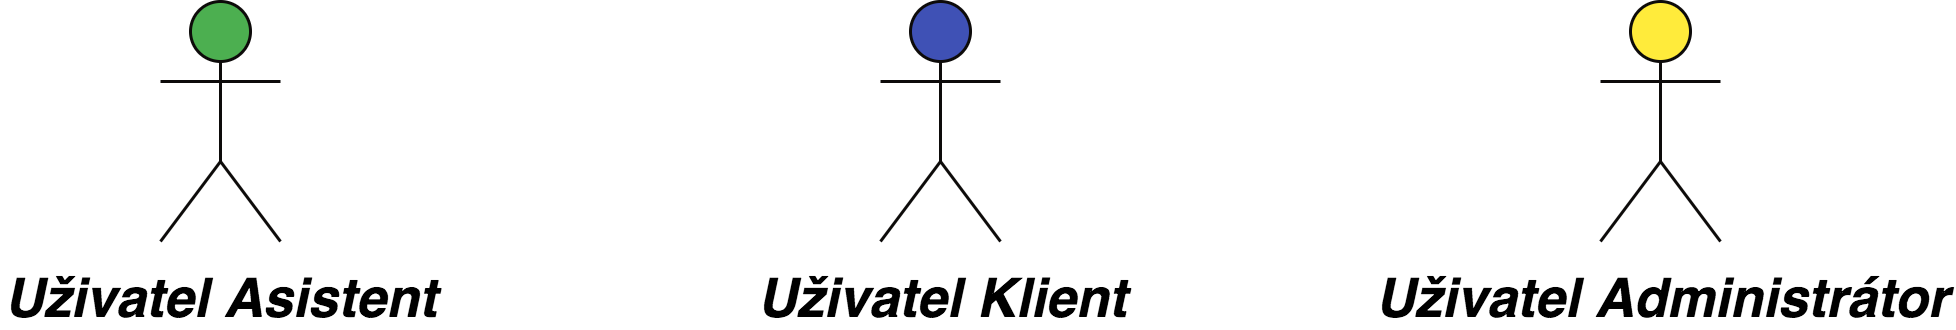
\includegraphics[scale=0.15]{img/actors.png}
        \caption{Aktéři systému}
        \label{fig:actors}
\end{figure}

\subsubsection{Uživatel Asistent}
Jedná se o aktéra, který je zároveň klientovi s mentálním postižením odborným asistentem,
jenž o něj pečuje a poskytuje mu podporu. Tento aktér je releventní k vytváření obsahu,
který má pomoci klientovi k lepší orientaci při cestování a také mu může připravenou
cestu předvést. Může také nahraná data editovat a případně je rozšiřovat. Může také zadat
do aplikace zadat své kontaktní údaje pro možnou nečekanou situaci klienta na cestách, případně
nastavit zálohování uložených dat pro zamezení jejich ztráty při ztrátě telefonu nebo jeho výměně
za jiný.

\subsubsection{Uživatel Klient}
Klient je osoba pro kterou je aplikace primárně určena a má mu pomoci vyřešit problém,
v tomto případě pomoci z orientací při cestování. Může si prohlížet obsah a zejména ho
využívat při cestách v terénu. Uživatel by měl být upozorněn na všechny uložené a rozeznané
data v závisloti na své pozici a měl by tak získat releventní informace k tomu, kde se právě
nachází. Dále může aplikaci využít ke snadnému kontaktování svého asistenta.

\subsubsection{Uživatel Administrátor}

\subsection{Use casy}
\label{labelx}
Pro uživatele klienta i asistenta jsou definovány případy užití zvlášť, neboť se celé chodvání
a použití aplikace bude v obou případech značně lišit.

\subsubsection{Uživatel asistent}
Pro uživatele asistnta jsou určeny složitější operace pro vytváření interaktivního obsahu pro klienta,
nastavování aplikace a prezentace klientovi. Pro use casy asistenta platí, že klient může těmto
krokům přihlížet, pokud o to projeví zájem.

\begin{figure}[H]
        \centering
                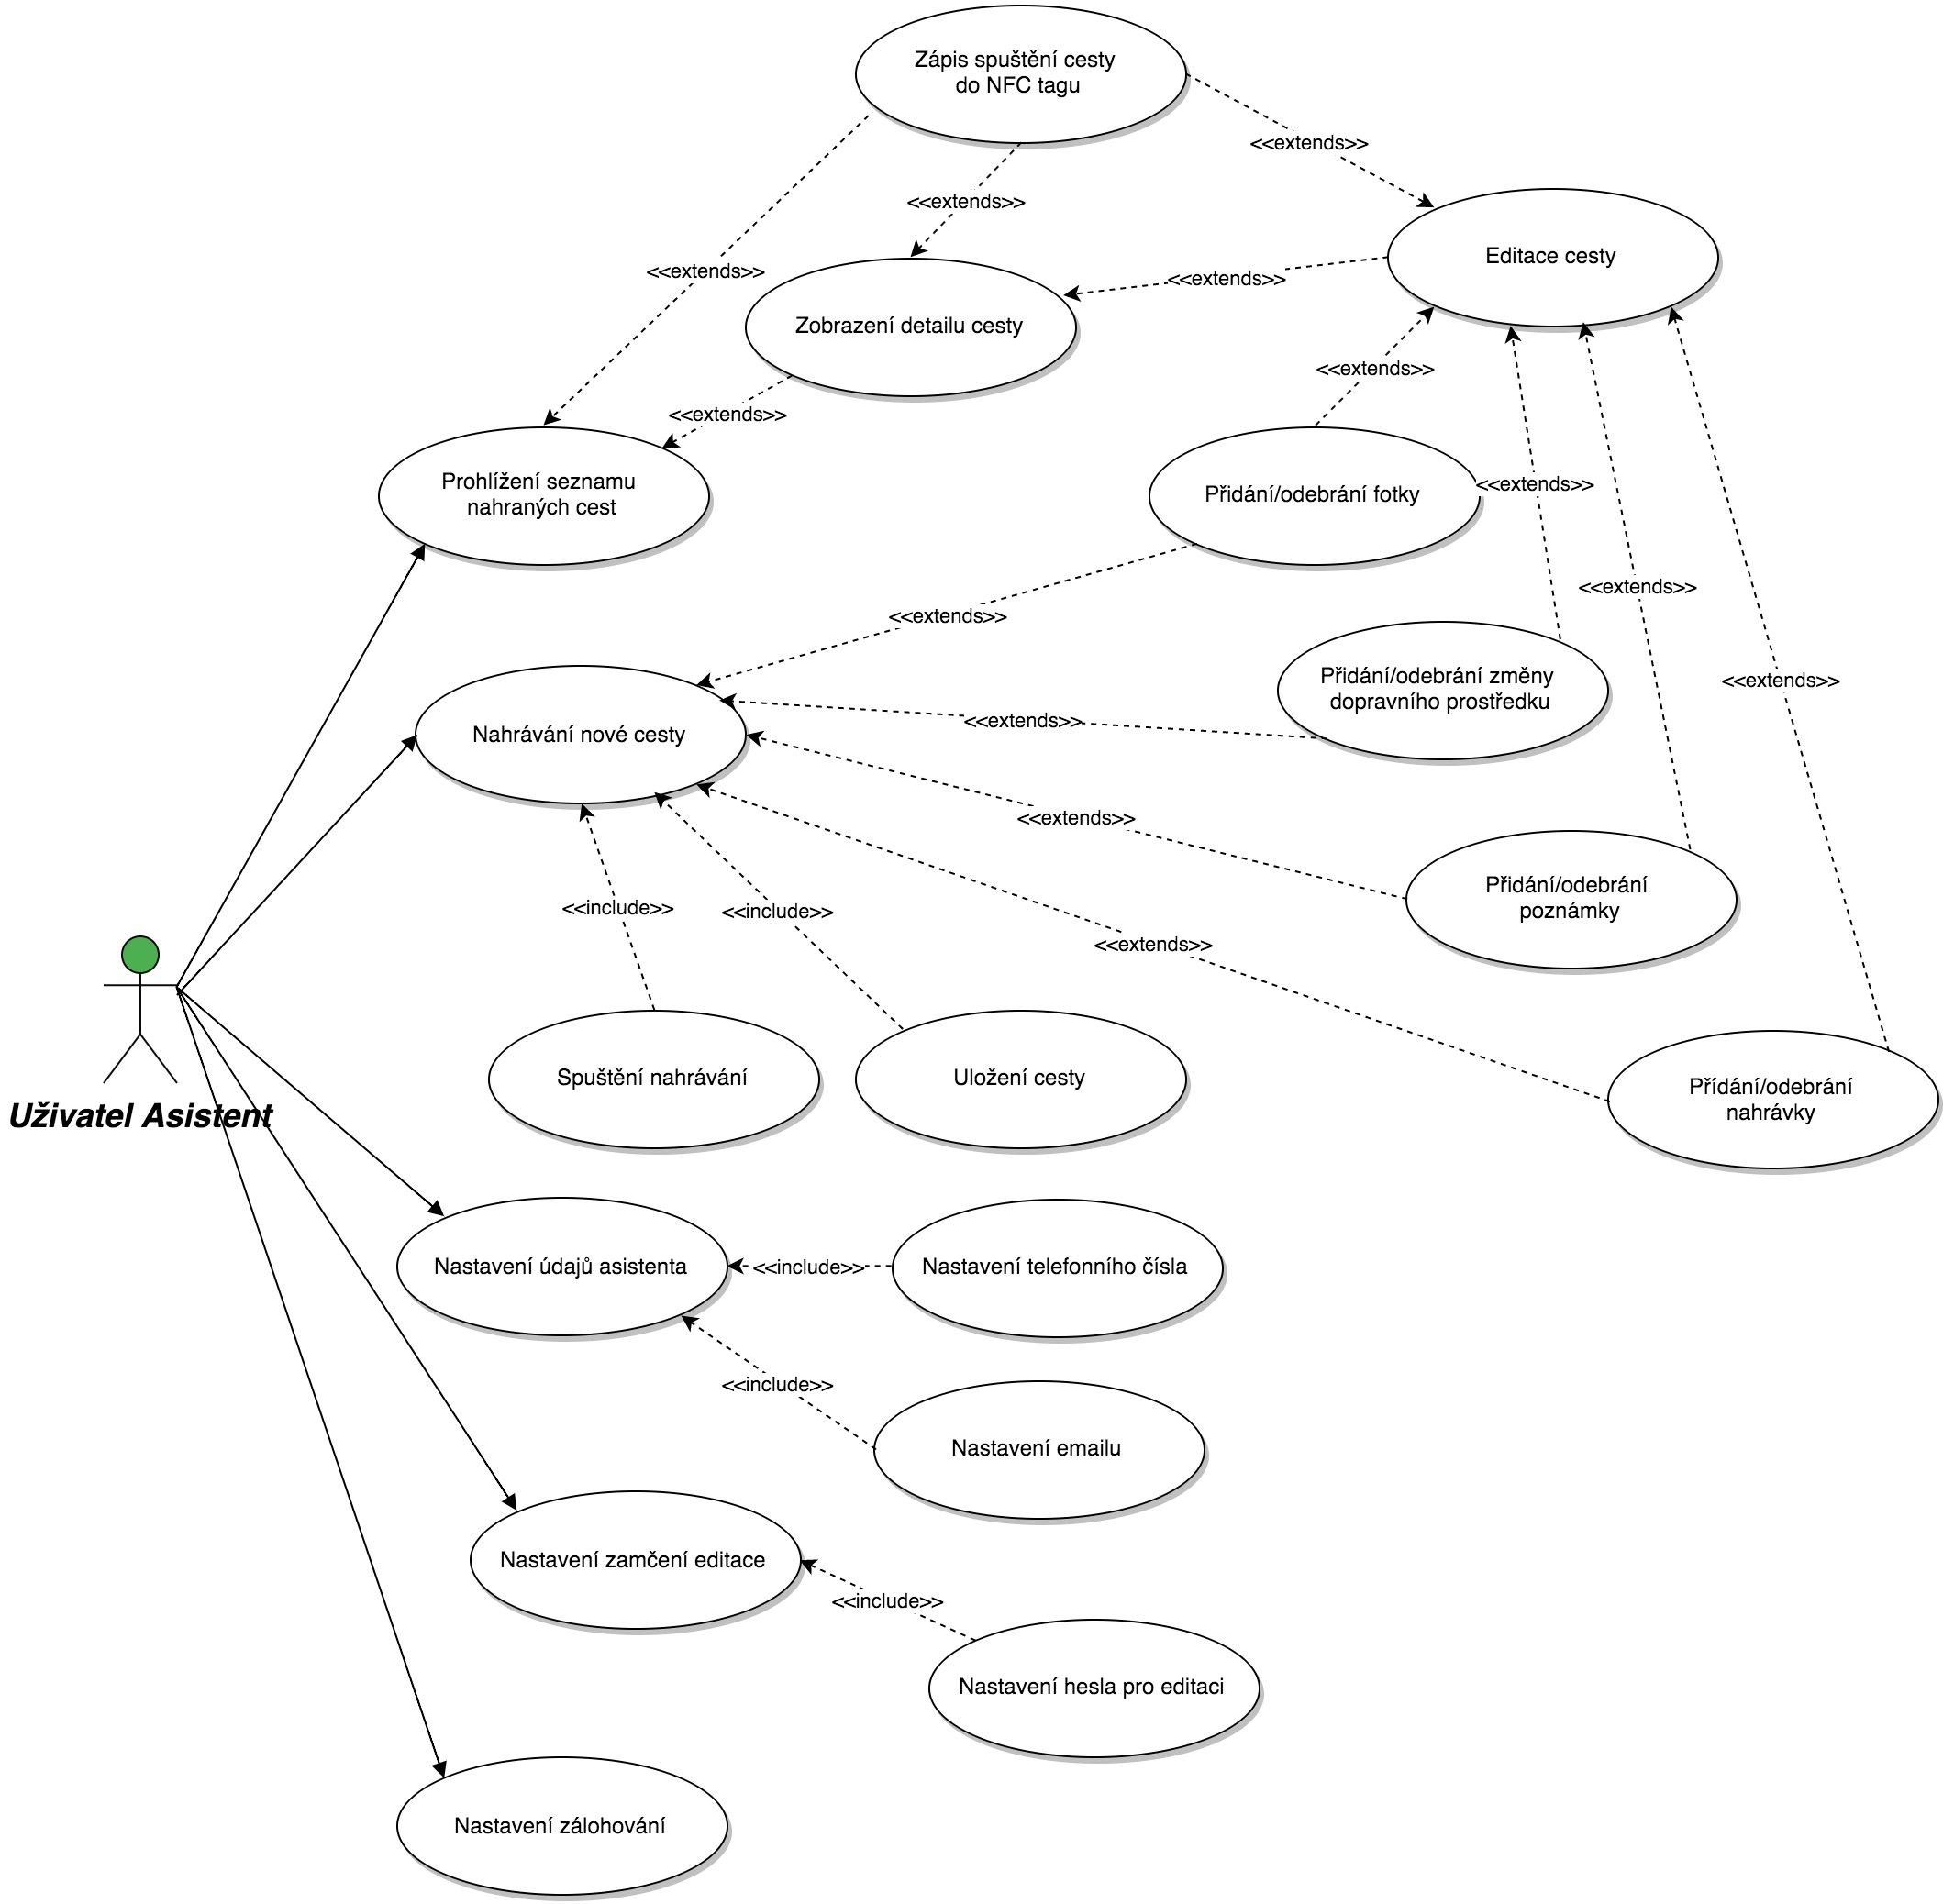
\includegraphics[scale=0.2]{img/UseCasesAsistant.png}
        \caption{Diagram use casů uživatele asistent}
        \label{fig:UseCasesAsistant}
\end{figure}
%
%\usecase{name}{label}
%\textbf{Aktéři:} Asistent
%
%\vspace{0.1cm}
%\noindent
%\textbf{Hlavní scénář:}
%
%\vspace{0.1cm}
%\noindent
%\textbf{Prekondice:}
%
%\vspace{0.1cm}
%\noindent
%\textbf{Spouštěč:}
%
%\vspace{0.1cm}
%\noindent
%\textbf{Rozšíření:}

\usecase{Prohlížení seznamu nahraných cest}{prohizeniasistent}
\textbf{Aktéři:} Asistent

\vspace{0.1cm}
\noindent
\textbf{Hlavní scénář:} Na úvodní obrazovce jsou zobrazeny všechny dosud nahrané cesty ve seznamu pod sebou.
Lze vidět pouze základní údaje a přiřazený obrázek pro snadnou orientaci. Uživatel se pomocí
kliknutí na řádek může podívat na celý detail cesty, případně pomocí rychlých akcí spustit ihned asistenci
a podobně.

\vspace{0.1cm}
\noindent
\textbf{Spouštěč:} Uživatel spustí aplikaci nebo se do ní vrátí pomocí notifikace v notifikační liště.

\vspace{0.1cm}
\noindent
\textbf{Rozšíření:}
\begin{itemize}
  \item \nameref{nahravanicesty}
  \item \nameref{detailasistent}
  \item \nameref{nfczapis}
\end{itemize}


\usecase{Zobrazení detailu cesty}{detailasistent}
\textbf{Aktéři:} Asistent

\vspace{0.1cm}
\noindent
\textbf{Hlavní scénář:} Uživateli se zobrazí detail cesty se všemi informacemi, ktré jsou o ní uloženy.
Na mapě si může prohlédnout kudy vedla, an místech fotografií jsou miniatury fotek, při změně dopravních
prostředků lze vidět ikony daných prostředků, zvukově a textové záznamy jsou označeny příslušnou ikonou.
Při klepnutí na indikátor některého z těchto záznamů se zobrazí jeho popis, který uživatel dříve zadal.
V detailu cesty lze poklepáním na tlačítko editovat přejít do módu editace cesty a všechny dříve zmíněné
záznamy upravit

\vspace{0.1cm}
\noindent
\textbf{Prekondice:} Cesta je uložena.

\vspace{0.1cm}
\noindent
\textbf{Spouštěč:} Uživatel klepne na řádek se zobrazenou cestou v seznamu cest.

\vspace{0.1cm}
\noindent
\textbf{Rozšíření:}
\begin{itemize}
  \item \nameref{editacecesty}
  \item \nameref{nfczapis}
\end{itemize}

\usecase{Zapsání cesty do NFC tagu}{nfczapis}
\textbf{Aktéři:} Asistent

\vspace{0.1cm}
\noindent
\textbf{Hlavní scénář:} Uživateli se zobrazí
obrazovka, která jej instruuje k přiložení NFC tagu k telefonu. Jakmile telefon zaznamená blízkost tagu,
zapíše do něj informaci o uložené cestě pro následné rychlé spouštění při přiložení tagu k telefonu.

\vspace{0.1cm}
\noindent
\textbf{Prekondice:} Cesta je uložena.

\vspace{0.1cm}
\noindent
\textbf{Spouštěč:} Uživatel klepne na ikonu NFC v detailu cesty nebo an rozšiřující menu v seznamu cest.


\usecase{Editace cesty}{editacecesty}
\textbf{Aktéři:} Asistent

\vspace{0.1cm}
\noindent
\textbf{Hlavní scénář:} Uživatel může editovat všechny uložné informace o cestě. Přepsání editačních
polí může změnit názvy a popis nahrané cesty, podržením a přetažením miniatur fotek nebo ikon dalších údajů na mapě může změnit
jejich pozici a tudíž místo, kdy se později vyvolají. Dále může podržením přetažením měnit tvar trasy,
při klepnutí na mapu přidat další záznamy. Jakmile je uživatel s editací spokojen, klepnutím na tlačíko
uložit se údaje zapíší do databáze a následující asistence cestování bude tyto údaje používat.

\vspace{0.1cm}
\noindent
\textbf{Prekondice:} Cesta je uložena.

\vspace{0.1cm}
\noindent
\textbf{Spouštěč:} Uživatel klepne na tlačítko editovat v detailu cesty.

\vspace{0.1cm}
\noindent
\textbf{Rozšíření:}
\begin{itemize}
  \item \nameref{pridanifotky}
  \item \nameref{pridaninahravky}
  \item \nameref{pridanipoznamky}
  \item \nameref{pridanizmenyprostredku}
    \item \nameref{odebranifotky}
    \item \nameref{odebraninahravky}
    \item \nameref{odebranipoznamky}
    \item \nameref{odebranizmenyprostredku}
\end{itemize}

\usecase{Přídání fotky}{pridanifotky}
\textbf{Aktéři:} Asistent

\vspace{0.1cm}
\noindent
\textbf{Hlavní scénář:} Spustí se fotoaparát zařízení a uživatel může začít fotit. Jakmile pořídí
fotografii, zobrazí se v aplikace okno pro zadání názvu fotky s dotazem pro uložení. Uživatel zadá název
a klepnutím na potvrzovací tlačítko se fotka uloží mezi data aplikace a zobrazí mezi aktuálními fotografiemi
na místě polohy uživatele v době pořízení fotografie.
\vspace{0.1cm}
\noindent
\textbf{Prekondice:} Uživatel nahrává nebo edituje cestu

\vspace{0.1cm}
\noindent
\textbf{Spouštěč:} Uživatel klepl na tlačítko přidat fotku

\usecase{Přídání zvukové nahrávky}{pridaninahravky}
\textbf{Aktéři:} Asistent

\vspace{0.1cm}
\noindent
\textbf{Hlavní scénář:} Uživateli se zobrazí obrazovka s textem mluvte a zvuk se zaznamenává.
Když je uživatel hotov, klepne na tlačítko stop a může nahrávce přidat název, který se bude později zobrazovat.
Poté tlačítkem nahrávku uloží mezi data aplikace s přiřazenou aktuální polohou uživatele.

\vspace{0.1cm}
\noindent
\textbf{Prekondice:} Uživatel nahrává nebo edituje cestu

\vspace{0.1cm}
\noindent
\textbf{Spouštěč:} Uživatel klepl na tlačítko přidat nahrávku

\usecase{Přídání poznámky}{pridanipoznamky}
\textbf{Aktéři:} Asistent

\vspace{0.1cm}
\noindent
\textbf{Hlavní scénář:} Uživateli se zobrazí okno s textovým vstupem a vysune se klávesnice. Uživatel
zadá textovou poznámku a po klepnutí na potvrzovací tlačítko se poznámka uloži s asociací k aktuální poloze
uživatele.

\vspace{0.1cm}
\noindent
\textbf{Prekondice:} Uživatel nahrává nebo edituje cestu

\vspace{0.1cm}
\noindent
\textbf{Spouštěč:} Uživatel klepl na tlačítko přidat poznámku

\usecase{Přídání změny dopravního prostředku}{pridanizmenyprostredku}
\textbf{Aktéři:} Asistent

\vspace{0.1cm}
\noindent
\textbf{Hlavní scénář:} Zobrazí se okno se nabídkou tlačítek s obrázkem dopravního prostředku.
Uživatel může zároveň přidat ke změně dopravního prostředku přidat popis. Po kliknutí na
tlačítko s dopravním prostředkem se změna dopravního prostředku uloží s asociovanou aktuální polohou
uživatele.

\vspace{0.1cm}
\noindent
\textbf{Prekondice:} Uživatel nahrává nebo edituje cestu

\vspace{0.1cm}
\noindent
\textbf{Spouštěč:} Uživatel klepl na tlačítko s aktuálním dopravním prostředkem.


\usecase{Nahrávání cesty}{nahravanicesty}
\textbf{Aktéři:} Asistent

\vspace{0.1cm}
\noindent
\textbf{Hlavní scénář:} Uživateli se zobrazí nahrávací okno, kde může vidět svou aktuální pozici
a po klepnutí na tlačítko nahrávat začne aplikace sbírat data o poloze a umožní mu přidávat další data
k právě nahrávené pozici. V notifikační liště se objeví notifikace o tom, že aplikace právě nahrává.
Uživatel může v tu chvíli odejít z aplikace, případně navštívit její jiné obrazovky a poté se do nahrávání vrátit,
aniž by ztratil právě nahrávaná data. Stejně tak po opuštění aplikace při nahrávání se do ní může vrátit
klepnutím na zobrazenou notifikaci.

Na mapě vidí uživatel dosud nahranou a uloženou cestu a případné přidané data.
Klepnutím na tlačítko uložit se aktuálně nahraní data a média uloží, případně aktualizují.
Pokud uživatel dokončil nahrávání cesty, klepne na tlačítko uložit a poté tlačítkem stop zastaví nahrávání,
notifikace zmizí a cesta je v seznamu cest připraveno pro spuštění asistence, případně následnou editaci.
Pokud uživatel ukončí nahrávání bez uložení, je na toto upozorněn a při potvrzení ukončení jsou nahraná data
smazána.

\vspace{0.1cm}
\noindent
\textbf{Prekondice:} Uživatel má v telefonu povolené získávání polohy pomocí GPS..

\vspace{0.1cm}
\noindent
\textbf{Spouštěč:} Uživatel klepne na tlačítko nahrávat v seznamu nahraných cest.

\vspace{0.1cm}
\noindent
\textbf{Rozšíření:}
\begin{itemize}
  \item \nameref{pridanifotky}
  \item \nameref{pridaninahravky}
  \item \nameref{pridanipoznamky}
  \item \nameref{pridanizmenyprostredku}
  \item \nameref{odebranifotky}
  \item \nameref{odebraninahravky}
  \item \nameref{odebranipoznamky}
  \item \nameref{odebranizmenyprostredku}
\end{itemize}


\usecase{Odebrání fotky}{odebranifotky}
\textbf{Aktéři:} Asistent

\vspace{0.1cm}
\noindent
\textbf{Hlavní scénář:} Uživateli se zobrazí okno s dotazem zda chce fotku odebrat. Po klepnutí na
potvrzovací tlačítko je fotka smazána z úložiště a odstraněna její miniatura z aktuální cesty.

\vspace{0.1cm}
\noindent
\textbf{Prekondice:} Uživatel nahrává nebo edituje cestu a má uloženou fotografii.

\vspace{0.1cm}
\noindent
\textbf{Spouštěč:} Uživatel podrží prst na miniatuře fotografie a vybere možnost smazat.



\usecase{Odebrání zvukové nahrávky}{odebraninahravky}
\textbf{Aktéři:} Asistent

\vspace{0.1cm}
\noindent
\textbf{Hlavní scénář:} Uživateli se zobrazí dotaz zda chce nahrávku opravdu smazat, po potvrzení
se uložená nahrávka odstraní a zmizí její ikona.

\vspace{0.1cm}
\noindent
\textbf{Prekondice:} Uživatel nahrává nebo edituje cestu a má uloženou nahrávku.

\vspace{0.1cm}
\noindent
\textbf{Spouštěč:} Uživatel podrží prst na ikoně nahrávky a vybere možnost smazat.



\usecase{Odebrání poznámky}{odebranipoznamky}
\textbf{Aktéři:} Asistent

\vspace{0.1cm}
\noindent
\textbf{Hlavní scénář:} Uživateli se zobrazí okno s dotazem na smazání poznámky. Po potvrzení se
nahrávka smaže a zmizí ikona indikující nahrávku.
\vspace{0.1cm}
\noindent
\textbf{Prekondice:} Uživatel nahrává nebo edituje cestu a má uloženou poznámku.

\vspace{0.1cm}
\noindent
\textbf{Spouštěč:} Uživatel podrží prst na ikoně poznámky a vybere možnost smazat.


\usecase{Odebrání změny dopravního prostředku}{odebranizmenyprostredku}
\textbf{Aktéři:} Asistent

\vspace{0.1cm}
\noindent
\textbf{Hlavní scénář:} Uživateli se zobrazí okno s dotazem na smazání změny dopravního prostředku.
Po potvrzení se nahrávka smaže a zmizí ikona indikující nahrávku.

\vspace{0.1cm}
\noindent
\textbf{Prekondice:} Uživatel nahrává nebo edituje cestu a má uloženou změnu dopravního prostředku.

\vspace{0.1cm}
\noindent
\textbf{Spouštěč:} Uživatel podrží prst na ikoně změny dopravního prostředku a vybere možnost smazat.


\usecase{Nastavení údajů asistenta}{nastaveniudaju}
\textbf{Aktéři:} Asistent

\vspace{0.1cm}
\noindent
\textbf{Hlavní scénář:} Uživateli se zobrazí obrazovka s nastavením údajů, kde může vyplnit své údaje.

\vspace{0.1cm}
\noindent
\textbf{Spouštěč:} Uživatel klepl na tlačítko nastavení.

\vspace{0.1cm}
\noindent
\textbf{Rozšíření:}
\begin{itemize}
  \item \nameref{nastavenicisla}
  \item \nameref{nastaveniemailu}
\end{itemize}

\usecase{Nastavení telefonního čísla asistenta}{nastavenicisla}
\textbf{Aktéři:} Asistent

\vspace{0.1cm}
\noindent
\textbf{Hlavní scénář:} Editovatelné pole pro telefonní číslo se zvýrazní a vysune se numerická klávesnice.
Uživatel zadá své telefonní číslo, které se automaticky formátuje do přívětivějšího formátu. Po ukončení
editace je telefonní číslo automaticky uloženo. Pokud telefonní číslo neodpovídá formátu telefonních čísel
v České Republice, uživatel je na toto upozorněn a je vyzván k úpravě vstupu.

\vspace{0.1cm}
\noindent
\textbf{Spouštěč:} Uživatel klepl na editační pole s telefonním číslem asistenta.


\usecase{Nastavení emailu asistenta}{nastaveniemailu}
\textbf{Aktéři:} Asistent

\vspace{0.1cm}
\noindent
\textbf{Hlavní scénář:} Editovatelné pole pro emailovou adresu se zvýrazní a vysune se klávesnice.
Uživatel zadá svou emailovou adresu. Po ukončení editace je emailová adresa automaticky uložena.
Pokud emailová adresa neodpovídá správnému formátu emailové adresy, uživatel je na toto upozorněn
a vyzván k úpravě vstupu.

\vspace{0.1cm}
\noindent
\textbf{Spouštěč:} Uživatel klepl na editovatelné pole emailové adresy.


\usecase{Nastavení zamčení editace}{nastavenizamceni}
\textbf{Aktéři:} Asistent

\vspace{0.1cm}
\noindent
\textbf{Hlavní scénář:} Uživateli se zobrazí editovatelné pole, kde může zadat heslo pro zamčení editace
obsahu aplikace. Pokud toto heslo nezadá, aplikace bue stále v módu edotace a uložená data bude možné upravit.
Uživatel zadá heslo, to bude uloženo a bude nyní vyžadováno pro zpřistupnění úprav cest, případně nastavení.

\vspace{0.1cm}
\noindent
\textbf{Spouštěč:} Uživatel klepl na tlačítko nastavení zamčení.

\usecase{Nastavení zálohování}{nastavenizalohovani}
\textbf{Aktéři:} Asistent

\vspace{0.1cm}
\noindent
\textbf{Hlavní scénář:} Uživateli se zobrazí výběr z listu zda chce zálohovat manuálně, jednou za den, týden
nebo za měsíc. Uživatel vybere jednu z možností a podle výběru se naplánují příslušné akce.

\vspace{0.1cm}
\noindent
\textbf{Prekondice:} Uživatel má na zařízení přidán Google účet.

\vspace{0.1cm}
\noindent
\textbf{Spouštěč:} Uživatel klepl na tlačítko nastavení zálohování.


















\subsubsection{Uživatel klient}
Pro klienta jsou určeny více intuitivní a nenáročné operace vyžadující co nejméně aktivních
kroků z klientovi strany. Aplikace by měla na základě polohy a dalších údajů sama rozpoznat,
co má v  danou chvíli udělat.

\begin{figure}[H]
        \centering
                \includegraphics[scale=0.2]{img/UseCasesClient.png}
        \caption{Diagram use casů uživatele klient}
        \label{fig:UseCasesClient}
\end{figure}










\subsection{Použité nástroje}
\subsubsection{draw.io (http://www.draw.io)}
Online nástroj pro tvorbu grafů, všech různých typů diagramů, myšlenkových map a dalších.
Celý edior běží pouze v prohlížeči a synchronizuje vytvářené grafy s připojeným úložištěm
Google Drive nebo Dropbox. Grafy jsou tak přístupné  a editovatelné odkudkoliv a aplikace
je opravdu pokročilá a při práci není vůbec poznat, že vše probíhá pouze v prohížeči.
Umožňuje sdílení i export zhotovených diagramů do mnoha formátů a je tedy velice snadné
sdílet a používat vytvořenou práci.
Nástroj byl použit pro vytváření use case diagramů a třídnách diagramů v této práci.
\begin{figure}[H]
        \centering
                
\includegraphics[scale=0.2]{img/drawiologo.png}
        \caption{Logo nástroje draw.io}
        \label{fig:iologo}
        \centering Zdroj: \url{http://www.draw.io}
\end{figure}

%\subsection{Podnadpis\footnote{Inspirace v \cite{saad}}}



\section{Závěr}


\begin{thebibliography}{99}

\end{thebibliography}

  \appendix

  \section{Zdrojové kódy}
  Kódy lze nalézt i na přiloženém CD.

\end{document}